\documentclass[9pt,twocolumn,twoside]{pnas-new}
% Use the lineno option to display guide line numbers if required.
% Note that the use of elements such as single-column equations
% may affect the guide line number alignment. 

\templatetype{pnasresearcharticle} % Choose template 
% {pnasresearcharticle} = Template for a two-column research article
% {pnasmathematics} = Template for a one-column mathematics article
% {pnasinvited} = Template for a PNAS invited submission

\title{Reported cases of alcohol-related domestic abuse increase following the victory of the England national football team}

% Use letters for affiliations, numbers to show equal authorship (if applicable) and to indicate the corresponding author
\author[a]{Anna Trendl}
\author[b]{Neil Stewart} 
\author[b]{Timothy Mullett}

\affil[a]{Department of Psychology, University of Warwick, CV4 7AL}
\affil[b]{Warwick Business School, University of Warwick, CV4 7AL}
%\affil[b]{Warwick Business School, University of Warwick, CV4 7AL}

% Please give the surname of the lead author for the running footer
\leadauthor{Lead author last name} 

% Please add here a significance statement to explain the relevance of your work
\significancestatement{Authors must submit a 120-word maximum statement about the significance of their research paper written at a level understandable to an undergraduate educated scientist outside their field of speciality. The primary goal of the Significance Statement is to explain the relevance of the work in broad context to a broad readership. The Significance Statement appears in the paper itself and is required for all research papers.}

% Please include corresponding author, author contribution and author declaration information
\authorcontributions{Please provide details of author contributions here.}
\authordeclaration{Please declare any conflict of interest here.}
\equalauthors{\textsuperscript{1}A.O.(Author One) and A.T. (Author Two) contributed equally to this work (remove if not applicable).}
\correspondingauthor{\textsuperscript{2}To whom correspondence should be addressed. E-mail: trendlak\@gmail.com}

% Keywords are not mandatory, but authors are strongly encouraged to provide them. If provided, please include two to five keywords, separated by the pipe symbol, e.g:
\keywords{domestic abuse $|$ football } 

\begin{abstract}
Previous research has suggested a link between large-scale televised sport tournaments and increased rates of reported domestic abuse\cite{Card2011}, \cite{Kirby2014}, but the role of alcohol in this relationship has not been explored. Using crime data from the third largest police force in England, serving a population of 2.9 million\cite{populationfigure}, we show that the number of reported alcohol-related domestic abuse cases increases by 61\% following an England victory in a national football tournament. The effect is driven by male to female alcohol-related cases, and is absent from male to male, female to male, and female to female cases. A three-hour analysis reveals that the increase starts in the three-hour period of the match, peaks in the three hours following the victory, and gradually declines to its baseline level 12 hours after the match. This temporal pattern, along with the random allocation of match days strongly indicates a causal effect of an England victory on alcohol-related domestic abuse. 
\end{abstract}

\dates{This manuscript was compiled on \today}
\doi{\url{www.pnas.org/cgi/doi/10.1073/pnas.XXXXXXXXXX}}

\begin{document}

% Optional adjustment to line up main text (after abstract) of first page with line numbers, when using both lineno and twocolumn options.
% You should only change this length when you've finalised the article contents.
\verticaladjustment{-2pt}

\maketitle
\thispagestyle{firststyle}
\ifthenelse{\boolean{shortarticle}}{\ifthenelse{\boolean{singlecolumn}}{\abscontentformatted}{\abscontent}}{}

% If your first paragraph (i.e. with the \dropcap) contains a list environment (quote, quotation, theorem, definition, enumerate, itemize...), the line after the list may have some extra indentation. If this is the case, add \parshape=0 to the end of the list environment.
\dropcap{``}If England gets beaten, so will she'' - read the poster as part of the ``The Not-So-Beautiful-Game'' awareness campaign launched by the National Centre for Domestic Violence in the wake of the 2018 FIFA World Cup \cite{NCDV}. While the link between sporting events and domestic abuse has been the focus of a number of smaller studies\cite{Williams2014}, large-scale quantitative investigations of this relationship are relatively scarce. The most extensive study in the topic found that an unexpected loss of the local National Football League (NFL) team resulted in a 10\% increase in the rate of reported male to female intimate partner violence (IPV) in the US\cite{Card2011}. 

In England, most studies have focused on the link between football (soccer) and domestic abuse. Football's history is inextricably linked to England, and it is by far the most popular sport in the country \cite{Parry2014}, with the 2018 World Cup attracting a record number of 44.5 million viewers\cite{BBC}. One of the earliest examinations of the link between football and domestic abuse used daily data from 33 out of 39 police forces in England from the period of June-July in 2009 and 2010 (World Cup tournament year)\cite{Brimicombe2012}. They tested whether the reported number of domestic abuse cases increased significantly on days when the England national football team won, lost, or drew, compared to the same days in 2009, and other, non-match days during the tournament in 2010. The study found that rates of reported domestic abuse increased significantly when England lost or won (about 33-35\%), but did not change on days when they drew. 

A more comprehensive investigation, using daily counts of domestic abuse in Lancashire from the 2002, 2006 and 2010 World Cup, found a 38\% increase in the number of reported domestic violence cases when the England team lost, and a 26\% increase when they won or drew\cite{Kirby2014}. These estimates had been widely discussed in the British media before the 2018 World Cup, and the figures were also quoted on the posters in the Not-So Beautiful Game Campaign. While domestic abuse is predominantly understood as a pattern of ongoing behaviour involving a series of occurrences, rather than a one-off incident triggered by football \cite{Brooks-Hay2018}, these studies, and other qualitative investigations\cite{Swallow} nevertheless suggest that national football tournaments can create an environment for abusers that is conducive to domestic abuse.

Why would national football tournaments, such as the World Cup or the European Championship precipitate domestic abuse? England's participation in these tournaments are times of heightened patriotic emotions and a strengthened sense of ``Englishness'', fuelled by media narratives that often use war references, and a ``us vs. them'' rhetoric to generate and represent an English national identity\cite{Vincent2014}. Previous qualitative research has suggested that televised contact sports can serve as vehicle for the male sports fan to redefine, and express his masculinity in a way that allows dominance, control, and can ultimately manifest in the perpetration of domestic abuse\cite{Sabo,Swallow}, given susceptibility to such behaviours. We speculate that this observation is especially pertinent in the context of England's participation in national football tournaments, owing to the popularity of the sport in the country, the associated media attention, and the resulting heightened sense of national consciousness.

Qualitative investigations suggest that alcohol can be a significant factor in the link between football and domestic abuse. Alcohol has a strong association with domestic abuse\cite{Peralta2010}: those with alcohol-problems are more likely to be perpetrators and, when alcohol is involved, there is evidence that the violence might result in more serious injuries. However, it is generally understood that the role of alcohol should be considered in the context of a range of social, biological and pyschological factors, and that alcohol is not the direct cause of domestic abuse \cite{Javaid2015,Peralta2010}. One explanation for the co-occurrence of domestic abuse and alcohol is that, for some men, drinking and violence plays an instrumental role in the construction and expression of masculinity, especially when the problem of masculine deficiency is present (e.g., by unemployment)\cite{Peralta2010}. It has also been suggested that some perpetrators use alcohol to deflect responsibility for their actions, using alcohol as a ``shield'' that protects them from being seen as a violent abuser\cite{Javaid2015}.  

In the US, the relationship between unexpected NFL losses and IPV did not depend on alcohol-involvement in the abuse case\cite{Card2011}, while England-based quantitative studies did not look at the role of alcohol in particular. Given the strong association between drinking culture and football in England\cite{Dixon2014}, a relationship continuously reinforced by the marketing practices of the alcohol industry\cite{Gornall2014}, we hypothesize that alcohol plays an important role in the relationship between national football tournaments and domestic abuse.

To explore this hypothesis, we test if the daily number of reported domestic abuse cases recorded by the West Midland Police in England between 2010 and 2018 increase on days when the England national team plays in the World Cup or the European Championship, and whether the effect, if any, depends on alcohol-involvement in the reported case or the result of the match. We find that alcohol-related domestic abuse significantly increases following an England victory. Our rich dataset further allows us to investigate various aspects of this win-effect, including the temporal pattern of the increase, and exploring whether the link between football and domestic abuse depends on the gender of the perpetrator and victim. We conduct various robustness checks of the win-effect. We also examine if the increase extends to other types of criminal behaviours apart from domestic abuse, and whether similar links exist between rugby and domestic abuse. Finally, we test if the abuse perpetrated on England match days is characteristically different from abuse occurring on non-match days.

In the UK, the term ``domestic abuse'' refers to a wide range of behaviours, from physical and sexual violence to psychological, emotional, financial abuse, threatening behaviour, stalking and harassment, either within a family or an intimate relationship\cite{ONS}. Recent changes to the definition introduced the concept of coercive control, which recognises domestic abuse as a pattern of incidents, which can include any of the above behaviours. Previous research has mostly focused on IPV, the largest subcategory of domestic abuse. While IPV is more common than abuse perpetrated by family members\cite{ONS}, our dataset does not contain information about the exact relationship between the victim and perpetrator, therefore we cannot separate the two types of abuse, and we will refer to them collectively as ``domestic abuse''.


Our dataset contains all cases of domestic abuse that have been reported to the West Midlands Police between 2010 and 2018, but the vast majority of all domestic abuse incidents in fact never get reported (according to the Crime Survey of England and Wales, only 17\% of all domestic abuse victims reported the abuse to the police between April 2017 and March 2018\cite{ONS}). This substantial reporting bias, and its potential correlation with other contextual factors warrants a careful interpretation of the estimates from any quantitative study investigating domestic abuse, and highlights the importance of utilising a mixed methods approach to explore the factors facilitating domestic abuse. 


%Note: please start your introduction without including the word ``Introduction'' as a section heading (except for math articles in the Physical Sciences section); this heading is implied in the first paragraphs. 

\section*{Guide to using this template on Overleaf}

Please note that whilst this template provides a preview of the typeset manuscript for submission, to help in this preparation, it will not necessarily be the final publication layout. For more detailed information please see the \href{http://www.pnas.org/site/authors/format.xhtml}{PNAS Information for Authors}.

If you have a question while using this template on Overleaf, please use the help menu (``?'') on the top bar to search for \href{https://www.overleaf.com/help}{help and tutorials}. You can also \href{https://www.overleaf.com/contact}{contact the Overleaf support team} at any time with specific questions about your manuscript or feedback on the template.

\subsection*{Author Affiliations}

Include department, institution, and complete address, with the ZIP/postal code, for each author. Use lower case letters to match authors with institutions, as shown in the example. Authors with an ORCID ID may supply this information at submission.

\subsection*{Submitting Manuscripts}

All authors must submit their articles at \href{http://www.pnascentral.org/cgi-bin/main.plex}{PNAScentral}. If you are using Overleaf to write your article, you can use the ``Submit to PNAS'' option in the top bar of the editor window. 

\subsection*{Format}

Many authors find it useful to organize their manuscripts with the following order of sections;  Title, Author Affiliation, Keywords, Abstract, Significance Statement, Results, Discussion, Materials and methods, Acknowledgments, and References. Other orders and headings are permitted.

\subsection*{Manuscript Length}

PNAS generally uses a two-column format averaging 67 characters, including spaces, per line. The maximum length of a Direct Submission research article is six pages and a PNAS PLUS research article is ten pages including all text, spaces, and the number of characters displaced by figures, tables, and equations.  When submitting tables, figures, and/or equations in addition to text, keep the text for your manuscript under 39,000 characters (including spaces) for Direct Submissions and 72,000 characters (including spaces) for PNAS PLUS.

\subsection*{References}

References should be cited in numerical order as they appear in text; this will be done automatically via bibtex, e.g. \cite{belkin2002using} and \cite{berard1994embedding,coifman2005geometric}. All references should be included in the main manuscript file.  

\subsection*{Data Archival}

PNAS must be able to archive the data essential to a published article. Where such archiving is not possible, deposition of data in public databases, such as GenBank, ArrayExpress, Protein Data Bank, Unidata, and others outlined in the Information for Authors, is acceptable.

\subsection*{Language-Editing Services}
Prior to submission, authors who believe their manuscripts would benefit from professional editing are encouraged to use a language-editing service (see list at www.pnas.org/site/authors/language-editing.xhtml). PNAS does not take responsibility for or endorse these services, and their use has no bearing on acceptance of a manuscript for publication. 

\begin{figure}%[tbhp]
\centering
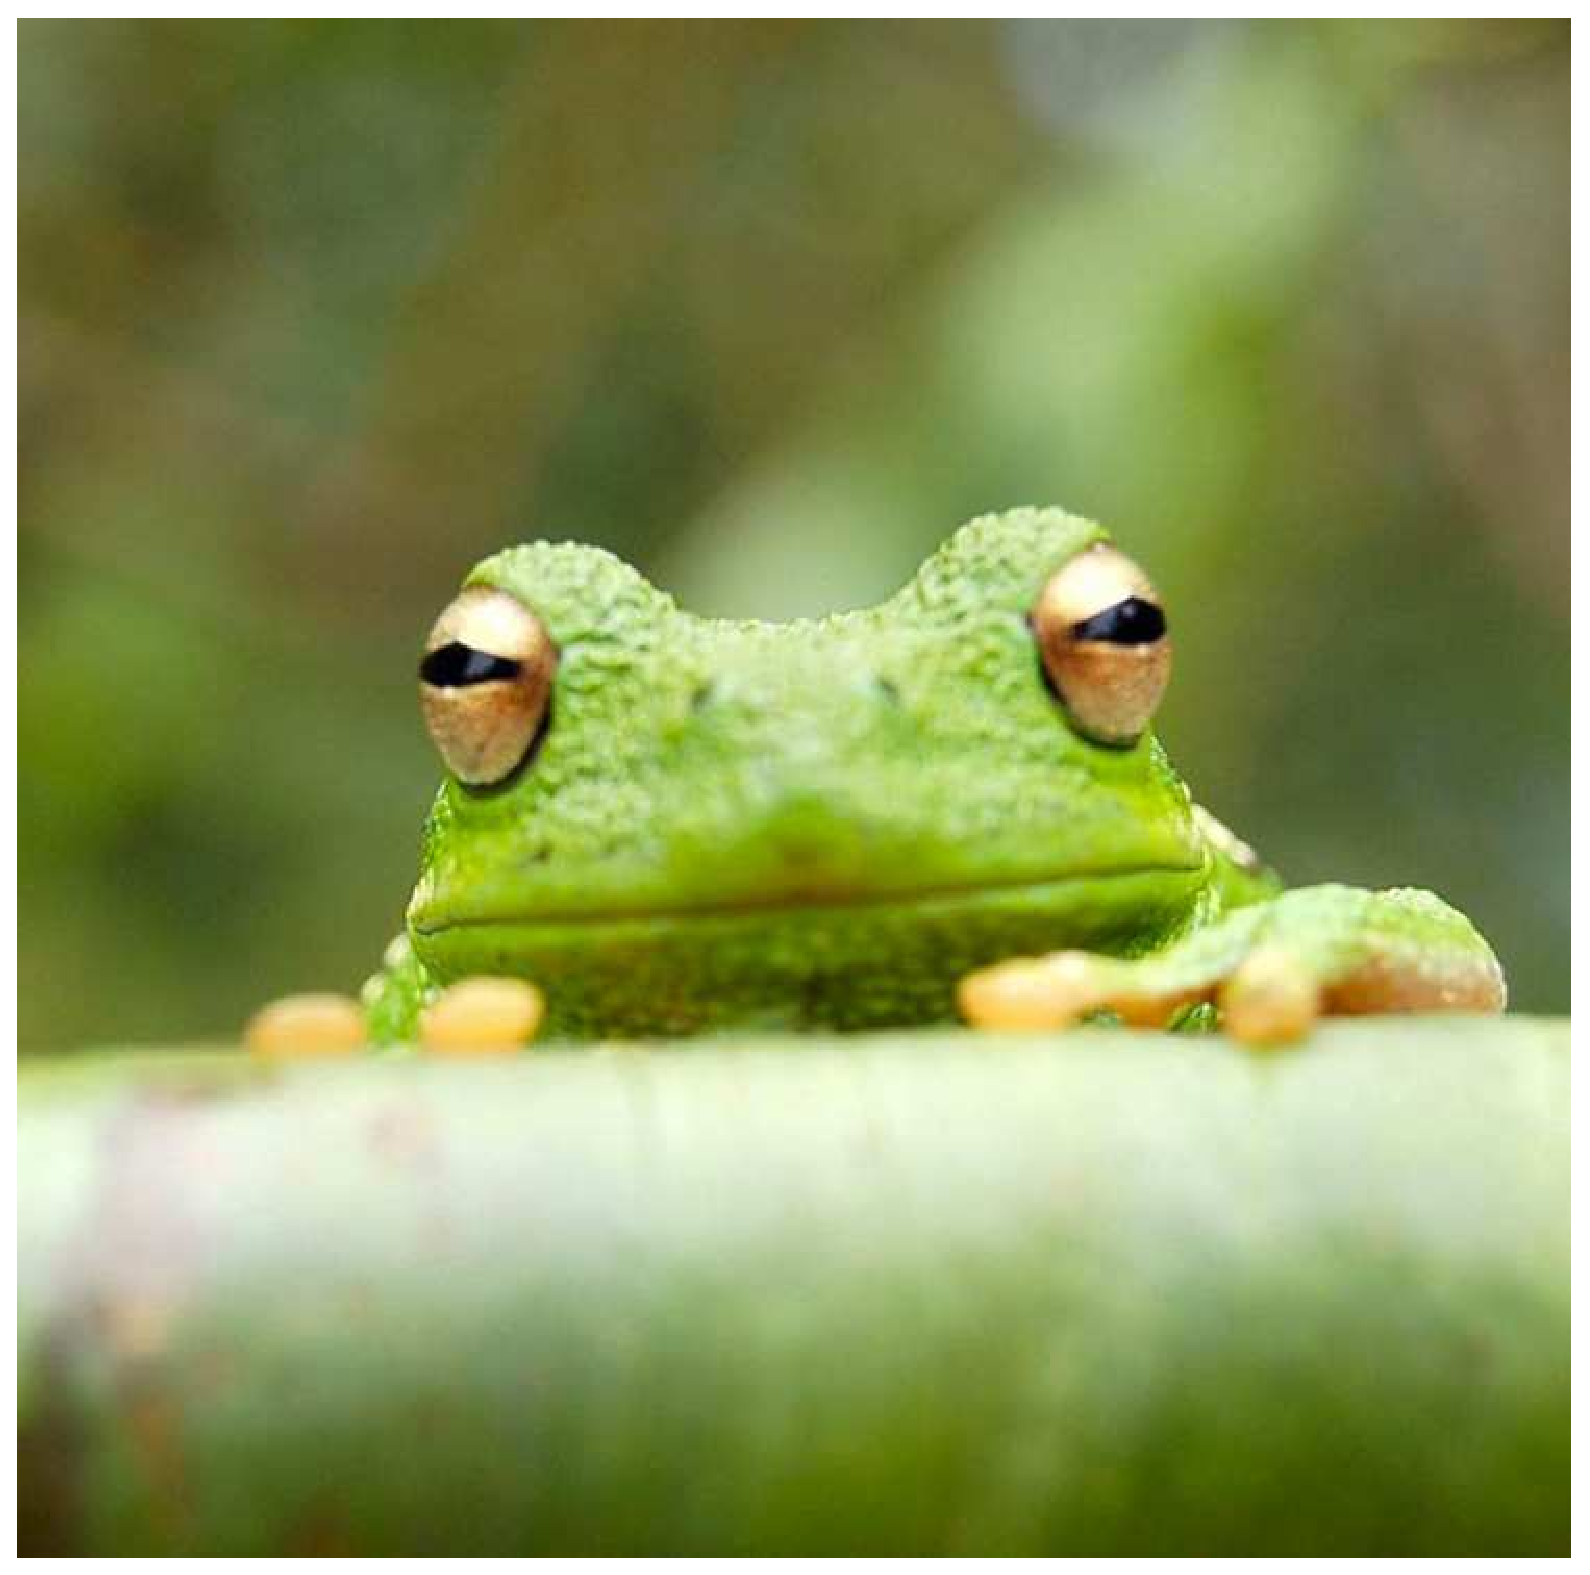
\includegraphics[width=.8\linewidth]{frog}
\caption{Placeholder image of a frog with a long example caption to show justification setting.}
\label{fig:frog}
\end{figure}


\begin{SCfigure*}[\sidecaptionrelwidth][t]
\centering
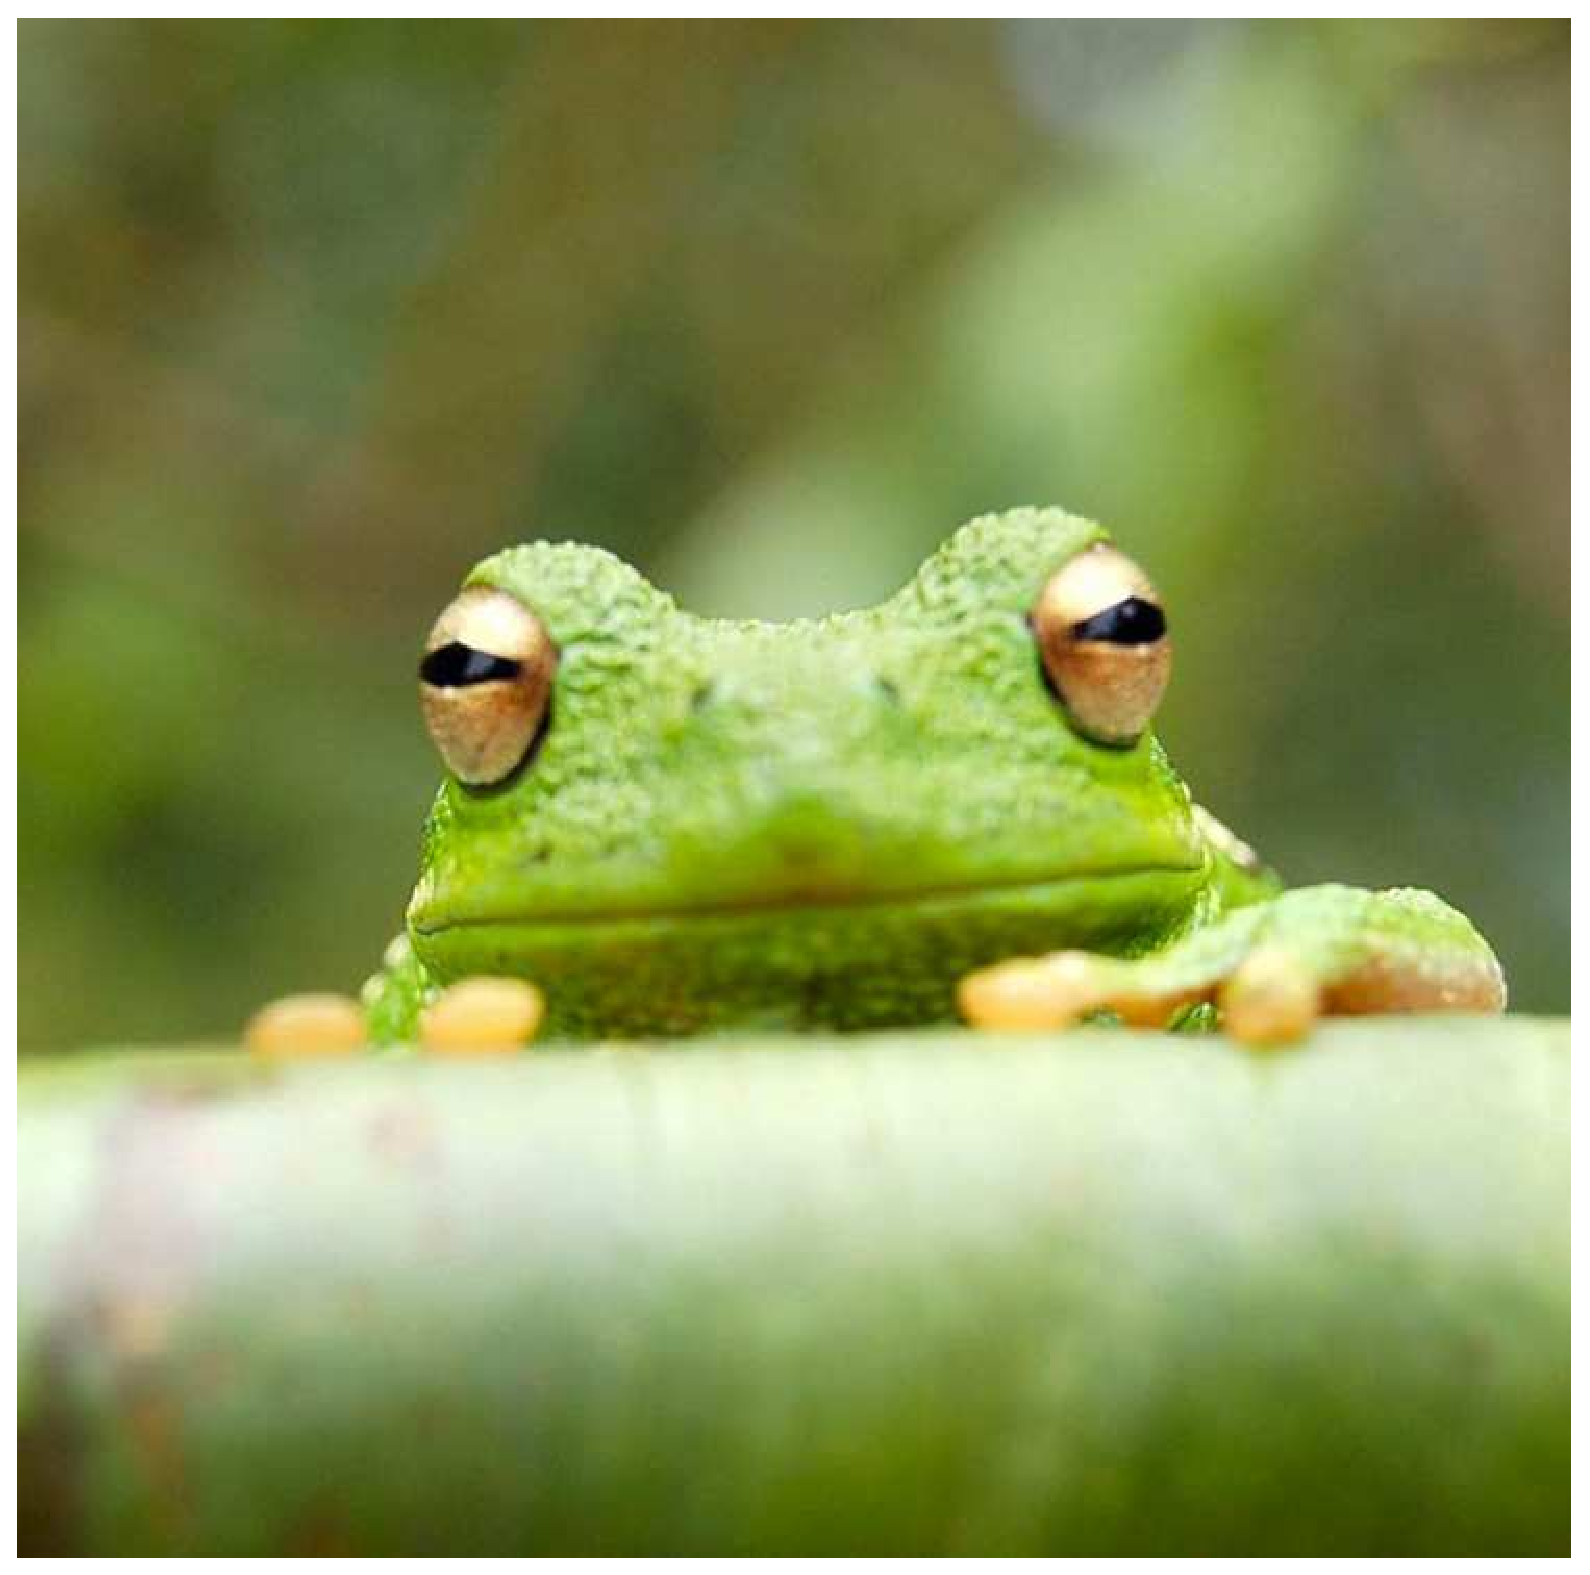
\includegraphics[width=11.4cm,height=11.4cm]{frog}
\caption{This caption would be placed at the side of the figure, rather than below it.}\label{fig:side}
\end{SCfigure*}

\subsection*{Digital Figures}
\label{sec:figures}

Only TIFF, EPS, and high-resolution PDF for Mac or PC are allowed for figures that will appear in the main text, and images must be final size. Authors may submit U3D or PRC files for 3D images; these must be accompanied by 2D representations in TIFF, EPS, or high-resolution PDF format.  Color images must be in RGB (red, green, blue) mode. Include the font files for any text. 

Figures and Tables should be labelled and referenced in the standard way using the \verb|\label{}| and \verb|\ref{}| commands.

Figure \ref{fig:frog} shows an example of how to insert a column-wide figure. To insert a figure wider than one column, please use the \verb|\begin{figure*}...\end{figure*}| environment. Figures wider than one column should be sized to 11.4 cm or 17.8 cm wide. Use \verb|\begin{SCfigure*}...\end{SCfigure*}| for a wide figure with side captions.

\subsection*{Single column equations}

Authors may use 1- or 2-column equations in their article, according to their preference.

To allow an equation to span both columns, options are to use the \verb|\begin{figure*}...\end{figure*}| environment mentioned above for figures, or to use the \verb|\begin{widetext}...\end{widetext}| environment as shown in equation \ref{eqn:example} below.

Please note that this option may run into problems with floats and footnotes, as mentioned in the \href{http://texdoc.net/pkg/cuted}{cuted package documentation}. In the case of problems with footnotes, it may be possible to correct the situation using commands \verb|\footnotemark| and \verb|\footnotetext|.

%% Do not use widetext if paper is in single column.
\begin{widetext}
\begin{align*}
(x+y)^3&=(x+y)(x+y)^2\\
       &=(x+y)(x^2+2xy+y^2) \numberthis \label{eqn:example} \\
       &=x^3+3x^2y+3xy^3+x^3. 
\end{align*}
\end{widetext}

\begin{table}%[tbhp]
\centering
\caption{Comparison of the fitted potential energy surfaces and ab initio benchmark electronic energy calculations}
\begin{tabular}{lrrr}
Species & CBS & CV & G3 \\
\midrule
1. Acetaldehyde & 0.0 & 0.0 & 0.0 \\
2. Vinyl alcohol & 9.1 & 9.6 & 13.5 \\
3. Hydroxyethylidene & 50.8 & 51.2 & 54.0\\
\bottomrule
\end{tabular}

\addtabletext{nomenclature for the TSs refers to the numbered species in the table.}
\end{table}

\subsection*{Supporting Information (SI)}

The main text of the paper must stand on its own without the SI. Refer to SI in the manuscript at an appropriate point in the text. Number supporting figures and tables starting with S1, S2, etc. Authors are limited to no more than 10 SI files, not including movie files. Authors who place detailed materials and methods in SI must provide sufficient detail in the main text methods to enable a reader to follow the logic of the procedures and results and also must reference the online methods. If a paper is fundamentally a study of a new method or technique, then the methods must be described completely in the main text. Because PNAS edits SI and composes it into a single PDF, authors must provide the following file formats only.

\subsubsection*{SI Text}

Supply Word, RTF, or LaTeX files (LaTeX files must be accompanied by a PDF with the same file name for visual reference).

\subsubsection*{SI Figures}

Provide a brief legend for each supporting figure after the supporting text. Provide figure images in TIFF, EPS, high-resolution PDF, JPEG, or GIF format; figures may not be embedded in manuscript text. When saving TIFF files, use only LZW compression; do not use JPEG compression. Do not save figure numbers, legends, or author names as part of the image. Composite figures must be pre-assembled.

\subsubsection*{3D Figures}

Supply a composable U3D or PRC file so that it may be edited and composed. Authors may submit a PDF file but please note it will be published in raw format and will not be edited or composed.

\subsubsection*{SI Tables}

Supply Word, RTF, or LaTeX files (LaTeX files must be accompanied by a PDF with the same file name for visual reference); include only one table per file. Do not use tabs or spaces to separate columns in Word tables.

\subsubsection*{SI Datasets} 

Supply Excel (.xls), RTF, or PDF files. This file type will be published in raw format and will not be edited or composed. 

\subsubsection*{SI Movies}

Supply Audio Video Interleave (avi), Quicktime (mov), Windows Media (wmv), animated GIF (gif), or MPEG files and submit a brief legend for each movie in a Word or RTF file. All movies should be submitted at the desired reproduction size and length. Movies should be no more than 10 MB in size. 

\subsubsection*{Still images}

Authors must provide a still image from each video file. Supply TIFF, EPS, high-resolution PDF, JPEG, or GIF files. 

\subsubsection*{Appendices}

PNAS prefers that authors submit individual source files to ensure readability. If this is not possible, supply a single PDF file that contains all of the SI associated with the paper. This file type will be published in raw format and will not be edited or composed.

\matmethods{Please describe your materials and methods here. This can be more than one paragraph, and may contain subsections and equations as required. Authors should include a statement in the methods section describing how readers will be able to access the data in the paper. 

\subsection*{Subsection for Method}
Example text for subsection.
}

\showmatmethods{} % Display the Materials and Methods section

\acknow{Please include your acknowledgments here, set in a single paragraph. Please do not include any acknowledgments in the Supporting Information, or anywhere else in the manuscript.}

\showacknow{} % Display the acknowledgments section

% \pnasbreak splits and balances the columns before the references.
% Uncomment \pnasbreak to view the references in the PNAS-style
% If you see unexpected formatting errors, try commenting out \pnasbreak
% as it can run into problems with floats and footnotes on the final page.
%\pnasbreak

% Bibliography
\bibliography{pnas-sample}

\end{document}